\documentclass[11pt,a4paper]{article}
\bibliographystyle{apalike}
\usepackage{epsfig, hyperref}
\usepackage{amsmath}
\usepackage{natbib}
\usepackage{listings}
\usepackage{color}

\definecolor{dkgreen}{rgb}{0,0.6,0}
\definecolor{gray}{rgb}{0.5,0.5,0.5}
\definecolor{mauve}{rgb}{0.58,0,0.82}

\lstset{frame=tb,
  language=Python,
  aboveskip=3mm,
  belowskip=3mm,
  showstringspaces=false,
  columns=flexible,
  basicstyle={\small\ttfamily},
  numbers=none,
  numberstyle=\tiny\color{gray},
  keywordstyle=\color{blue},
  commentstyle=\color{dkgreen},
  stringstyle=\color{mauve},
  breaklines=true,
  breakatwhitespace=true,
  tabsize=3
}

\begin{document}

\title{IDL to Python ``cheat sheet''}
\author{Nicholas P. Ross}
\date{\today}
\maketitle


% Usually omit these for ApJ or MNRAS style files:
%\tableofcontents
%\listoffigures
%\listoftables

\begin{abstract}
I've been keen to have an IDL to Python ``Cheat Sheet'' for some time. 
This is it. 
\end{abstract}

\section{Real basics}
    \subsection{iPython}
     $>$ conda update ipython

    \subsection{Versions}
    {\tt > python
      
      Python 2.7.6 |AnacondaCE 1.3.1 (x86\_64)| (default, Jan 10 2014, 11:23:15) 
      [GCC 4.0.1 (Apple Inc. build 5493)] on darwin 
      Type "help", "copyright", "credits" or "license" for more information. 
      
      \noindent
      >>> import numpy \\
      >>> print numpy.\_\_version\_\_ \\

      1.8.2 \\
      \noindent
      >>> import astropy \\
      >>> print astropy.\_\_version\_\_ \\

      0.4.1 \\
      \noindent
     >>> import sys\\ 
     >>> print (sys.version) \\

     2.7.10 (default, Oct 23 2015, 18:05:06) \\
     \lbrack GCC 4.2.1 Compatible Apple LLVM 7.0.0 (clang-700.0.59.5)]
     }

    \subsection{iPython from Fernando Perez}
    Try: tmpnb.org  {\bf VERY USEFUL}\\
    \href{http://www.pythonforbeginners.com/basics/ipython-a-short-introduction}{http://www.pythonforbeginners.com/basics/ipython-a-short-introduction}

    \subsection{Notebook}
    Click on the NBviewer...\\
    Then you can see the e.g. html of the notebook. \\
    But to change/execute it, then all you have to do is click the download button...\\
    Then put it on gitHub/Dropbox etc...\\
    (I need to learn about ``Tmox'' and ``SCreen'' Terminal emulators...)\\
  
    \noindent
    {\bf Run a code cell using Shift-Enter} or \\
    Alt-Enter runs the current cell and inserts a new one below.
    Ctrl-Enter run the current cell and enters command mode. 

    \noindent
    Google: ``ipython beyond plain python''\\
    
    http://nbviewer.ipython.org/github/fperez/cit2013/blob/master/06-IPython\%20-\%20beyond\%20plain\%20Python.ipynb

    iPython NB power = power of python + power of the command line with ``!'' + ``\%'' and ``\%\%'' ``magics''... 
    
http://nbviewer.ipython.org/github/ipython/ipython/blob/1.x/examples/notebooks/Part\%204\%20-\%20Markdown\%20Cells.ipynb

\begin{figure}
  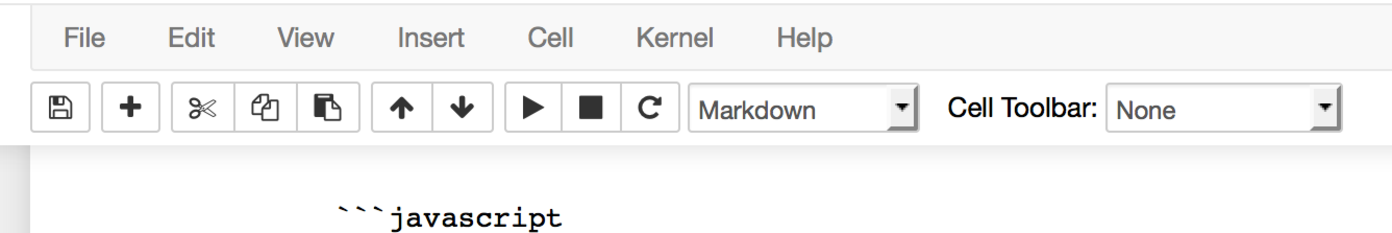
\includegraphics[height=4.0cm,width=14.0cm]
{iPython_NB_toolbar.pdf}
      \centering
      \caption[]
              {Clicking on the Cell Toolbar ``Code'', ``Markdown'' etc. will power what happens in the Clells!!!}
      \label{fig:fig1}
    \end{figure}

\href{https://github.com/profjsb/python-bootcamp}{https://github.com/profjsb/python-bootcamp}



\section{Britton's Classes :-)}

\subsection{``If lost in the desert...''}
$>>>$ dir(thing) \\
$>>>$ dir(thing) \\

%% http://tex.stackexchange.com/questions/45981/square-brackets-in-math-mode-without-the-bracket-symbols

\subsection{Lists}
\begin{lstlisting}
$>>>$ super_list = [0, [3,4,5], "Hello World!", range(5)] 
$>>>$ print super\_list 

[0, [3, 4, 5], 'Hello World!', [0, 1, 2, 3, 4]] 
$>>>$ print super\_list[1] 
%+ - = ! / ( ) [ ] < > | ' :
\lbrack3, 4, 5] 
$>>>$ print super\_list[-1]
\lbrack0, 1, 2, 3, 4] 
$>>>$ print super\_list[1[0]] 
Traceback (most recent call last):
  File "<stdin>", line 1, in <module>
TypeError: 'int' object is not subscriptable
$>>>$ print super\_list[1][0] 
  3

$>>>$ c = range(10) \\
$>>>$ print c \\
\lbrack0, 1, 2, 3, 4, 5, 6, 7, 8, 9]\\
$>>>$ c.append(range(3)) \\
$>>>$ print c \\
\lbrack0, 1, 2, 3, 4, 5, 6, 7, 8, 9, [0, 1, 2]]\\
$>>>$ c.extend(range(3)) \\
$>>>$ print c \\
\lbrack0, 1, 2, 3, 4, 5, 6, 7, 8, 9, [0, 1, 2], 0, 1, 2]\\
$>>>$ del c[4]\\
$>>>$ print c\\
%[0, 1, 2, 3, 5, 6, 7, 8, 9, [0, 1, 2], 0, 1, 2]\\


%\vspace{12pt}
$>>>$ z =  [42]*5\\
$>>>$ [42, 42, 42, 42, 42]\\

%\vspace{12pt}
$>>>$ print super\_list
[0, [3, 4, 5], 'Hello World!', [0, 1, 2, 3, 4]]
$>>>$ print len(super\_list)
4
$>>>$ print len(super\_list[-1])
5
\end{lstlisting}






%Section heading
\section{IDL to Python}
Key links:\\
\href{http://www.johnny-lin.com/cdat_tips/tips_array/idl2num.html}{IDL to Numeric/numarray Mapping}\\
\href{http://www.astro.umd.edu/~mbk/idl-numpy.html}{NumPy for IDL users}\\


\begin{table}
  \begin{center}
    \setlength{\tabcolsep}{4pt}
    \begin{tabular}{ll}
      \hline\hline
      IDL code   & Python code \\
      \hline
      data=READFITS('file',header) 	 & data=pyfits.open('file')\\
      tdata  = mrdfits('SpIESch1ch2.fits',0, hdr) 	 & tdata = data[0].data \\
      tbdata = mrdfits('SpIESch1ch2.fits',1, hdr) 	 & tdata = data[1].data \\
      help, tbdata, /str     & info(tbdata)\\
      print, size(tbdata)  & shape(tbdata)\\
      print, tbdata[0].flux\_aper\_1 & print tbdata.FLUX\_APER\_1[0]\\
      help, tbdata.flux\_aper\_1        & tbdata.FLUX\_APER\_1? \\
      fluxaper = tbdata.flux\_aper\_1[2] & fluxaper = ??? \\
      \hline 
     {\it (using fitsio)} & d = fitsio.read('SpIESch1ch2.fits',1) \\
      \hline
      \label{tab:IDL2Python}
    \end{tabular}
    \caption{IDL to Python}
  \end{center}
\end{table}



\section{INPUT}


\section{OUTPUT}
For the ``write'' statement, I think you have to put everything into 
a string format, otherwise it just barfs... \\

\noindent
\begin{lstlisting}
  outfile = open('WISE\_spectra\_triples\_4wget\_temp.dat', 'w') \\
for i in range(len(ra)): 

    print i, ra[i] 

    plate\_out = str(plate[i])

    mjd\_out = str(mjd[i]) 

    fiberid\_out = str(fiberid[i])

    outfile.write(plate\_out+"/spec-"+plate\_out+"-"+mjd\_out+"-"+fiberid\_out.zfill(4)+".fits \textbackslash n")
\end{lstlisting}






\section{IDL Where...}


\section{v2 vs. v3}
\subsection{print}
print a vs. print (a)
Thus, just use () all the time!!

\subsection{Division}
/ = truncating (integer floor) division in P2.x when using ints; float division in P3.x
// = truncating div in P2.x, P3.x 



\section{Linear Algebra}
\href{http://docs.scipy.org/doc/scipy/reference/tutorial/linalg.html}{http://docs.scipy.org/doc/scipy/reference/tutorial/linalg.html}


\begin{lstlisting}
import numpy as np
from scipy import linalg
A = np.array([[1,2],[3,4]])
linalg.inv(A)
A.dot(linalg.inv(A)) #double check
\end{lstlisting}



\section{Gotchas}
``follow up: PYTHONPATH is a hazardous environment variable, and should never include one Python's site-packages'' 
%% <blockquote class="twitter-tweet" lang="en"><p><a href="https://twitter.com/npr247">@npr247</a> <a href="https://twitter.com/jakevdp">@jakevdp</a> <a href="https://twitter.com/demitrimuna">@demitrimuna</a> follow up: PYTHONPATH is a hazardous environment variable, and should never include one Python\&#39;s site-packages</p>\&mdash; Min RK (@minrk) <a href="https://twitter.com/minrk/status/555137558850453505">January 13, 2015</a></blockquote><script async src="//platform.twitter.com/widgets.js" charset="utf-8"></script>

See 429 in history\_20150113.txt and onwards... :-) 

%> echo \$PYTHONPATH 
%:/Users/npr1/boss/products/Darwin/sdss3tools/v1_7_4/python:/cos_pc19a_npr/BOSS/esutil/esutil/lib/python2.7/site-packages/:/cos_pc19a_npr/BOSS/pydl/:/Users/npr1/boss/products/eups/bin



\section{A few General Notes}
    \subsection{What's the difference between raw\_input() and input()?}
    The difference is that {\tt raw\_input()} does not exist in Python 3.x,
    while {\tt input()} does. Actually, the old {\tt raw\_input()} has been renamed to
     {\tt input()}, and the old  {\tt input()} is gone (but can easily be simulated by
    using  {\tt eval(input())}).
    Reference: \href{http://stackoverflow.com/questions/4915361/whats-the-difference-between-raw-input-and-input-in-python3-x}{http://stackoverflow.com/questions/4915361/whats-the-difference-between-raw-input-and-input-in-python3-x}. 
   
 
\section{A few general notes and commands}
    \subsection{join()}
    Description: The method {\tt join()} returns a string in which the string elements of sequence have been joined by str separator.\\
    Syntax: Following is the syntax for {\tt join()} method: {\tt str.join(sequence)}. \\
    Parameters: sequence -- This is a sequence of the elements to be joined. \\
    Example: 
    \begin{lstlisting}
   s = "-";
   seq = ("a", "b", "c"); # This is sequence of strings.
   print s.join( seq )
   a-b-c
  \end{lstlisting}

    \subsection{eval()}  
    The eval function lets a python program run python code within itself.
    \begin{lstlisting}
   x = 1
   eval('x + 1')
   2
   eval('x')
   1
  \end{lstlisting}
    \begin{lstlisting}
   l
   [5, 5]
   cmd
   'insert(0,5)'
   eval("l."+cmd)
   print l
  [5, 5, 5]
  \end{lstlisting}



 

\section*{General Wee Tips}
Need points that are evenly spaced on a log scale? Use {\tt np.logscale(start, stop, base)} \\
By convention, matplotlib is imported as mpl. Also by convention, matplotlib.pyplot is imported as plt.\\




\section*{Useful Resources}
Borrows, begs and steals from: \\
http://www.astro.umd.edu/$sim$mbk/idl-numpy.html\\
http://www.johnny-lin.com/cdat\_tips/tips\_array/idl2num.html\\
http://www.astrobetter.com/idl-vs-python/ \\
http://www.astrobetter.com/wiki/tiki-index.php?page=Python+Switchers+Guide \\
http://mathesaurus.sourceforge.net/idl-numpy.html
http://www.scicoder.org/mapping-idl-to-python/

\noindent
Also, 
http://www.cv.nrao.edu/~aleroy/pytut/topic2/intro\_fits\_files.py

\noindent





\end{document}

